\documentclass{beamer}
\usepackage{graphicx}
\usepackage{amsmath}      % for \lVert \rVert, etc.
\usetheme{CambridgeUS}

\title{Koopman Control via Nyström Kernel Approximation}
\author{Muthana Alsaadi}
\institute[University of Al-Nahrain]{College of Information Engineering\\University of Al-Nahrain}
\date{September 2025}
\logo{
\includegraphics[height=1cm]{coie.jpeg}}

\AtBeginSection[]
{
  \begin{frame}[allowframebreaks]
    \frametitle{Table of Contents}
    \tableofcontents[currentsection]
  \end{frame}
}

\begin{document}

\frame{\titlepage}

\begin{frame}[allowframebreaks]{Table of Contents}
  \tableofcontents
\end{frame}

% ---------------------------
\section{Introduction}

\begin{frame}{Introduction: Why Can't a Robot Fold a T-Shirt?}
\begin{block}{Problem}
Why can a robot build a car with precision, but can't fold a t-shirt?
\end{block}
\end{frame}

\subsection{Defining the Challenge: Nonlinear Chaos}

\begin{frame}{Defining the Challenge: Nonlinear Chaos}
The problem isn't the robot's strength or precision; it's the nature of the object—it's an unpredictable floppy mess.

\bigskip
\begin{tabular}{|p{4cm}|p{6cm}|}
\hline
Linear Systems (Simple) & Nonlinear Systems (Chaos) \\ \hline
Predictable. Analogous to pushing a ball down a ramp.
& Unpredictable. Analogous to a piece of cloth falling through the air. A tiny input can lead to a massive unexpected output. \\ \hline
\end{tabular}
\end{frame}

\subsection{The Breakthrough Solution \& Key Wins}
\begin{frame}{The Breakthrough Solution \& Key Wins}
\begin{itemize}
  \item We combine the Koopman operator framework with kernel methods.
  \item We introduce the Nyström approximation to handle the computational complexity, acting as a ``good enough shortcut''.
\end{itemize}
\begin{block}{The Big Deal}
The approximated Riccati operator converges at rate $\mathbf{m^{-1/2}}$, and the LQR objective converges at rate $\mathbf{m^{-1}}$, where $m$ is the random subspace size.
\end{block}
\end{frame}

\begin{frame}{Summary Diagram}
\begin{figure}
  \centering
  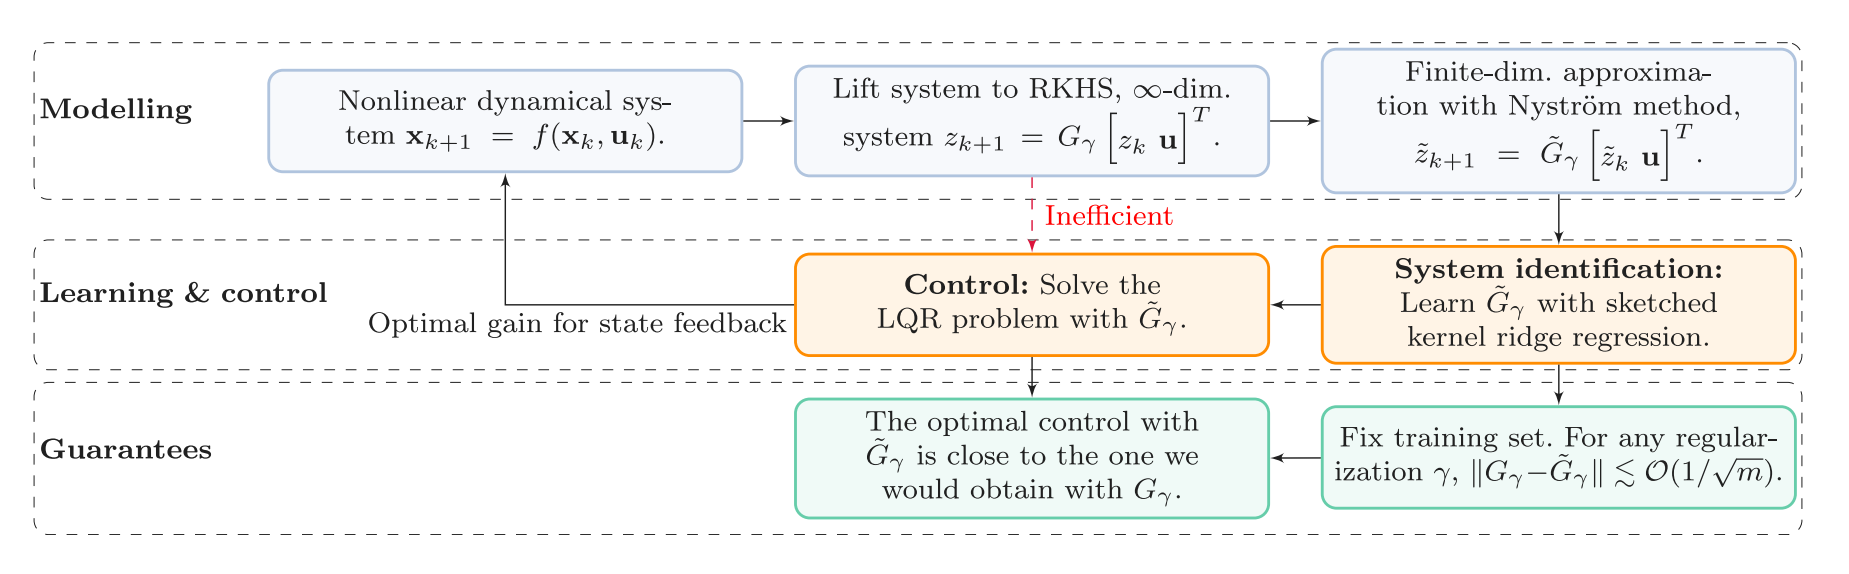
\includegraphics[width=\linewidth]{summary.png}
  \caption{Given controls and trajectories of a nonlinear system, kernels build a linear, data-driven model. Kernel inversions are made tractable via Nyström.}
\end{figure}
\end{frame}

% ---------------------------
\section{Prerequisite Knowledge}

\subsection{Systems Notation (Formalizing the Chaos)}
\begin{frame}{Systems Notation (Formalizing the Chaos)}
\begin{itemize}
  \item Discrete dynamics: $x_{t+1} = f(x_t, u_t)$.
  \item Affine-in-input focus: $f(x,u)=g(x)+Bu$.
  \item Augmented state $w$: combining state $x$ and input $u$.
\end{itemize}
\end{frame}

\subsection{The Koopman Operator Framework}
\begin{frame}{The Koopman Operator (The Magic Trick)}
\begin{itemize}
  \item The Koopman operator transforms our view of the system (not the system itself).
  \item It lifts behavior via nonlinear observables $\xi$.
  \item In the lifted space the dynamics appear linear.
  \begin{block}{Definition}
    $(K\xi)(w_t)=\xi(w_{t+1})$.
  \end{block}
\end{itemize}
\end{frame}

\subsection{Reproducing Kernel Hilbert Spaces (RKHS)}
\begin{frame}{Reproducing Kernel Hilbert Spaces (RKHS) \\ (The Infinite Stage)}
\begin{itemize}
  \item To get a perfect linear viewpoint, observables live in an RKHS $H$.
  \item RKHS can be infinite-dimensional and act as universal approximators.
\end{itemize}
\begin{alertblock}{Challenge}
Computers cannot handle infinity.
\end{alertblock}
\end{frame}

\subsection{Linear Quadratic Regulator (LQR)}
\begin{frame}{Linear Quadratic Regulator (LQR) (The Engineer's Tool)}
\begin{itemize}
  \item Once dynamics are linear (in the lifted space), apply LQR.
  \item Minimize a quadratic objective over an infinite horizon.
  \item Has an analytic solution: state-feedback gain $K$ via DARE.
\end{itemize}
\end{frame}

\subsection{Quiz 1 (Prerequisites Check)}
\begin{frame}{Quiz 1 (Prerequisites Check)}
\begin{block}{Q1}
How does the Koopman operator turn nonlinear dynamics into linear ones?
\end{block}
\begin{block}{Q2}
Why do standard control methods fail on truly nonlinear systems like soft cloth?
\end{block}
\end{frame}

% ---------------------------
\section{System Identification \& The Nyström Shortcut}

\subsection{The RKHS: The Challenge of the ``Infinite Stage''}
\begin{frame}[allowframebreaks]{The RKHS: The Challenge of the ``Infinite Stage''}
\begin{itemize}
  \item The Koopman operator works in an RKHS ($H_1$) that contains observables $\psi(x)$ needed to linearize the behavior.
\end{itemize}

\begin{block}{The Cheat Sheet Analogy}
The RKHS is like an infinite ``cheat sheet'' containing every possible feature—too big to compute exactly.
\end{block}

\framebreak

\begin{alertblock}{Problem}
Modeling perfectly would require processing infinite information. We need a finite surrogate.
\end{alertblock}

\begin{block}{Formalizing the Lift}
We lift with $\phi(w)$ into $H_1$ (keeping $u$ linear) and seek an operator $G_\gamma$ such that $z_{t+1}=G_\gamma \phi(w_t)$.
\end{block}
\end{frame}

\subsection{Kernel Methods and The Nyström Approximation}
\begin{frame}[allowframebreaks]{Kernel Methods and The Nyström Approximation: Making Infinity Finite}
\begin{itemize}
  \item \textbf{Kernel Methods:} Represent the infinite space $H_1$ while retaining universality.
  \item \textbf{Nyström Shortcut:} A randomized approximation to compute efficiently.
\end{itemize}

\framebreak

\begin{block}{The Random Survey Analogy}
Select $m$ landmark data pairs (``representative voters''): $\tilde{x}_{\text{in}}, \tilde{x}_{\text{out}}$.
\end{block}

\begin{itemize}
  \item \textbf{Dimensionality Reduction:} Project dynamics onto finite, data–dependent subspaces to get an approximate operator $\widetilde{G}_\gamma$.
\end{itemize}
\end{frame}

\subsection{Vector Dynamics and Efficiency}
\begin{frame}[allowframebreaks]{Vector Dynamics and Efficiency: The Computable Map}
\begin{itemize}
  \item Even with Nyström, $z_{t+1}=G_\gamma \phi(w_t)$ lives in function space; we need vectors.
  \item \textbf{The $m\times m$ Breakthrough:} Obtain a finite autoregressive model for coordinates $\tilde{z}$ that only needs inverting an $m\times m$ matrix.
\end{itemize}

\framebreak

\begin{block}{Rubik's Cube Analogy}
Nyström reduces a ``billion-layer'' cube to an $m\times m$ puzzle—huge computational savings.
\end{block}

\begin{itemize}
  \item \textbf{State Reconstruction:} Reconstruct $x$ from $z$ using a regularized least-squares estimate to define $C$.
\end{itemize}
\end{frame}

% ---------------------------
\section{Practical Implementation and LQR Formulation}

\subsection{The Two LQR Problems}
\begin{frame}[allowframebreaks]{The Two LQR Problems (The Ideal vs.\ The Real)}
\begin{block}{Recap}
We now have a finite, vector-valued representation of the dynamics; we can apply LQR.
\end{block}
\begin{block}{LQR Goal}
Minimize a quadratic cost penalizing state error and control effort.
\end{block}

\begin{enumerate}
  \item \textbf{Exact Dynamics LQR (Ideal):} Solve with the original (infinite-dimensional) RKHS dynamics—perfect but intractable.
  \item \textbf{Approximated Dynamics LQR (Real):} Solve with Nyström-approximated vector dynamics, yielding the stabilizing gain $K$.
\end{enumerate}

\framebreak

\begin{block}{God-like Controller Analogy}
The ideal LQR ``knows everything''; the approximated LQR is the fast, effective controller we can actually build.
\end{block}
\end{frame}

\subsection{Defining the Final Control Input}
\begin{frame}{Defining the Final Control Input (Putting the Gain to Work)}
\begin{itemize}
  \item The approximated LQR gives the optimal gain $K$.
  \item Apply $K$ back to the true state $x_k$ of the nonlinear system.
  \item Final control law: $\mathbf{u_k = K\,\Pi_{\text{out},x}\,\psi(x_k)}$.
\end{itemize}
\begin{block}{Steering Wheel Analogy}
Compute $K$ in the simple (linear) surrogate; feed it to the real nonlinear system to steer it.
\end{block}
\end{frame}

\subsection{The Full Pipeline}
\begin{frame}{The Full Pipeline (A 3-Step Recipe for Chaos Control)}
\begin{enumerate}
  \item \textbf{Sample Landmarks:} Select $m$ input/output landmarks from training data.
  \item \textbf{Compute the Map:} Use landmarks to compute efficient vector dynamics (only invert an $m\times m$ matrix).
  \item \textbf{Find the Steer:} Use these dynamics to solve LQR and get the optimal gain $K$.
\end{enumerate}
\end{frame}

\subsection{Quiz 2 (Control Loop Check)}
\begin{frame}{Quiz 2 (Control Loop Check)}
\begin{block}{Q1}
Why can problems (22) and (24) be treated as equivalent for LQR, though one is in function space and the other in vectors?
\end{block}
\begin{block}{Q2}
With $n=10{,}000$ and $m=100$ landmarks, what dictates the complexity of inverting the matrix for (18b)?
\end{block}
\end{frame}

% ---------------------------
\section{Theoretical Analysis: The Hard Proof that the Shortcut Works}

\subsection{Setting the Stage}
\begin{frame}{Setting the Stage: Necessary Assumptions}
To guarantee the LQR problem is well-posed, we need standard stability conditions:
\begin{enumerate}
  \item \textbf{Bounded Kernel:} The RKHS kernel $k$ is bounded.
  \item \textbf{Stabilizability:} The approximated dynamics can be driven to zero with suitable feedback.
  \item \textbf{Detectability:} Unstable modes are observable through the LQR cost.
  \item \textbf{Technical Riccati Condition:} $\sigma_{\min}(P)\ge 1$ (often satisfied by rescaling $Q$ and $R$).
\end{enumerate}
\end{frame}

\subsection{Accuracy of the Transition Operator 
  \texorpdfstring{$G_\gamma$}{G\_gamma}}
\begin{frame}{Accuracy of the Transition Operator 
  \texorpdfstring{$G_\gamma$}{G\_gamma}}
\begin{block}{Theorem 5 (Convergence Rate for 
  \texorpdfstring{$G_\gamma - \widetilde{G}_\gamma$}{G\_gamma - Gtilde})}
This bounds the error between the true infinite-dimensional dynamics ($G_\gamma$) and the Nyström shortcut ($\widetilde{G}_\gamma$).
\end{block}

\begin{block}{The Result}
The error converges proportional to $\mathbf{m^{-1/2}}$.
\end{block}

\begin{block}{Rule Book Analogy}
If we quadruple $m$, the operator error roughly halves. The rate applies to components too:
$\lVert A - \widetilde{A}\rVert$ and $\lVert B - \widetilde{B}\rVert$.
\end{block}
\end{frame}

\subsection{Convergence of the Riccati Operator 
  \texorpdfstring{$\widetilde{P}$}{Ptilde}}
\begin{frame}[allowframebreaks]{Convergence of the Riccati Operator 
  \texorpdfstring{$\widetilde{P}$}{Ptilde}}
\begin{block}{Recap}
  The Riccati operator $P$ solves the Discrete-Time Algebraic Riccati Equation (DARE) and determines the LQR gain $K$.
\end{block}

\begin{block}{Lemma 6 (Convergence Rate for $\widetilde{P} - P$)}
  This shows that the error in the optimal control strategy ($\widetilde{P}$ vs.\ $P$) is also bounded by $\mathcal{O}(\epsilon)$.
\end{block}

\framebreak

\begin{block}{The Result}
  Since $\epsilon$ is $m^{-1/2}$, the Riccati operator converges at rate $\mathbf{m^{-1/2}}$.
\end{block}

\begin{block}{Significance}
  This confirms that as our model improves at a predictable rate, the optimal control strategy derived from it improves at the same rate.
\end{block}
\end{frame}

\subsection{The Ultimate Test}
\begin{frame}[allowframebreaks]{The Ultimate Test: Convergence of the LQR Objective Function 
  \texorpdfstring{$\hat{J}$}{Jhat}}
  
  \begin{block}{The Setup}
    We compare the true optimal cost ($J$, using perfect dynamics) with the cost ($\hat{J}$) achieved when applying the Nyström-derived control gain $\widetilde{K}$ to the exact dynamics.
  \end{block}

  \begin{block}{Theorem 8 (Convergence Rate for $\hat{J} - J$)}
    The error between the costs is bounded proportionally to $g(\epsilon)^2$.
  \end{block}

  \framebreak

  \begin{block}{The Big Result}
    The final LQR objective function (total cost of effort and deviation) converges faster, at rate $\mathbf{m^{-1}}$.
  \end{block}

  \begin{block}{Why Faster?}
    The error in cost is proportional to the square of the operator error (where $g(\epsilon)=m^{-1/2}$).  
    This quadratic relationship means the performance measure improves much quicker as we increase $m$.
  \end{block}

\end{frame}

\subsection{Quiz 3 (Theory Check)}
\begin{frame}{Quiz 3 (Theory Check)}
    \begin{block}{Q1}
         If we double the number of Nyström landmarks ($m$), how much does the theoretical error on the LQR objective cost ($J$) decrease? (Answer: $O(m^{-1})$, so it approximately halves the error.)
    \end{block}
    \begin{block}{Q2}
        What technical adjustment must be made to the LQR weights ($Q, R$) to ensure Assumption 4 ($\sigma_{\min}(P) \ge 1$) is fulfilled?
    \end{block}
\end{frame}

% ---------------------------
\section{Conclusion and Future Frontiers}

\subsection{Recap of the Big Wins}
\begin{frame}{Recap of the Big Wins (The Summary)}
    \begin{enumerate}
        \item \textbf{Brilliant Combination:} Successfully paired the Koopman framework, reproducing kernels, and the Nyström method to design linear control for nonlinear systems.
        \item \textbf{Computational Efficiency:} The Nyström approximation achieved huge computational savings while preserving accuracy.
        \item \textbf{Theoretical Guarantee:} Provided the first theoretical proof that this approach is stable and reliable for control, with the LQR objective cost converging at rate $\mathbf{m^{-1}}$.
        \item \textbf{Proven Performance:} Tamed hard problems, including dynamic cloth manipulation.
        \item \textbf{Open Science:} The implementation is publicly available and open-source.
    \end{enumerate}
\end{frame}

\subsection{Future Frontiers}
\begin{frame}{Future Frontiers (Where Do We Go Next?)}
    This research significantly improves our ability to give robots the tools they need to handle soft, chaotic, and complex things.
    \begin{block}{Possibilities}
    What new frontiers could smart robots finally be ready to take on?
    \begin{enumerate}
        \item Delicate manufacturing?
        \item Autonomous surgery?
        \item Creative fields like art and sculpture?
    \end{enumerate}
    \end{block}
\end{frame}

\subsection{Final Quiz}
\begin{frame}{Final Quiz (Assessment)}
  \begin{block}{Q1}
    List the convergence rates derived in the theoretical analysis for  
    (1) the transition operator $\widetilde{G}_\gamma$  
    and (2) the final LQR objective cost $J$.
  \end{block}

  \begin{block}{Q2}
    Based on the numerical results, which feature representation 
    (Nyström, Splines, or Eigenfunctions) proved most robust for the Duffing oscillator when the number of features $m$ was small?
  \end{block}
\end{frame}

% ---------------------------
\section{Resources}

\subsection{Reference Paper}
\begin{frame}{Reference Paper}
    \textit{Edoardo Caldarelli, Antoine Chatalic, Adrià Colomé, Cesare Molinari, Carlos Ocampo-Martinez, Carme Torras, Lorenzo Rosasco,  
    Linear quadratic control of nonlinear systems with Koopman operator learning and the Nyström method,  
    Automatica, Volume 177, 2025, 112302, ISSN 0005-1098,  
    \url{https://doi.org/10.1016/j.automatica.2025.112302}}
    \begin{figure}
        \centering
        
\includegraphics[width=0.25\linewidth]{paper_code.png}
        \caption{QR code redirecting to the scientific journal referenced.}
    \end{figure}
\end{frame}

\subsection{Full Presentation}
\begin{frame}{Full Presentation}
    Get the full Beamer \LaTeX{} code from my GitHub repository:
    \begin{figure}
        \centering
        
\includegraphics[width=0.25\linewidth]{repo.png}
        \caption{QR code linking to the repository with the full presentation source.}
    \end{figure}
\end{frame}

\end{document}
